\chapter{Introduction}
Randomization is defined to be the study of making something 
random, which can be mathematically defined as :

\begin{definition}
    dFor a function $\mathcal{G} : \mathcal{D} \rightarrow \mathcal{R}$, 
    if $\mathcal{G}$ is random, then :\\
    \begin{equation*}
        P(\mathcal{G}(x) = y) = \frac{1}{\|\mathcal{R}\|}
    \end{equation*}
\end{definition}

\noindent The definition above says that the probability 
function for any input x to give an output y is uniformly 
random. 
\\\\
For a sequence of random numbers generated, two properties 
must hold :
\begin{itemize}
    \setlength\itemsep{0.01em}
    \item The values are uniformly distributed over a defined interval
    \item It is impossible to predict future values based on the past or present ones
\end{itemize}

\begin{note} 
    aAll the definitions provided here is for a function 
    to give a random output, which is what the report will be 
    focussing on.
\end{note}
\section{Importance of Randomness}
\subsection{Cryptography}
One of the most important use of random numbers is in 
cryptography. Cryptography is a study of techniques for 
secure communication in presence of third party adversary.
Formulation and explaination of a cipher can easilty explain 
the requirement of random numbers.
\\\\
A general communication channel looks as follows:
\begin{center}
    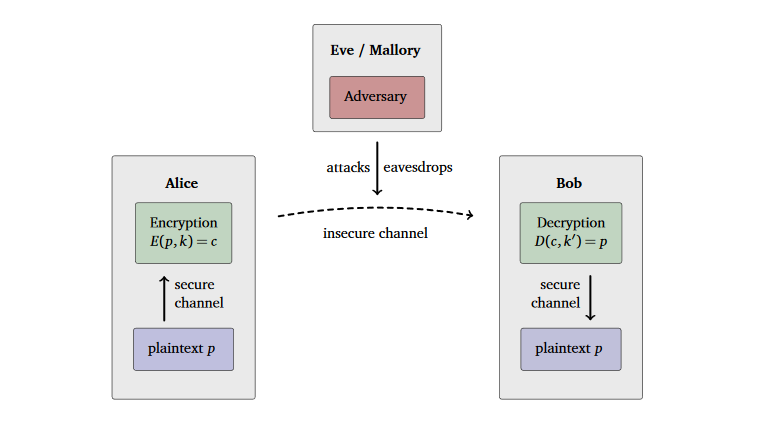
\includegraphics[scale=0.5]{img/abe_comm.png}
\end{center}

\noindent In this it can be seen that $c$, which is the 
ciphertext contains more information (higher entropy) than 
$m$ but has no intrinsic meaning in itself. Therefore, 
it can be anything.
\\\\
$E(m,k)$ is often randomized, in the case that even 
if the system is faulty and gets the same $m$ and $k$, 
the ciphertext $c$ will not be the same, thus protecting 
the information.
\\\\
Thus, $E(m)$ is a random number generator, which is why 
random number generators are important in the field of 
cryptography.

\subsection{Monte Carlo}
Another important application of random number generation is 
in Monte Carlo simulation methods. Monte Carlo methods are set 
of algorithms that repeatedly use random sampling to obtain 
deterministic results.
\\\\
One of the simplest and most used example of a Monte Carlo 
simulation problem is the determination of the value of $\pi$.
The code to calculate is as below:

\lstinputlisting[basicstyle=Large,style=py]{code/pi_mc.py}

\noindent From this, it can be seen that a deterministic value 
($\pi$) is being found using random sampling of x and y points.
\section{Pseudorandomness}
Any algorithm that exists is a set of defined steps that will 
always give a deterministic output. Therefore, generation of 
true random numbers is impossible for a normal computer algorithm.
\\\\
Rather if for the required amount of length, the sequence appears 
to be stastically random, then the job is done. An algorthm that 
provides with that kind of sequences are known as psuedo random 
number generators.
\\\\
An example of one such function is :
\begin{equation*}
    \mathcal{G}(x) = g^x \mod m
\end{equation*}

\noindent In this, the parameters are $g$ and $m$. This 
is a psuedo random number generator in the sense that if 
a predictive (non random) sequence of numbers are input as $x$, 
then the output sequence will appear to be random.
\\\\
The general structure of a psuedo random number generator is 
as follows:

\begin{center}
    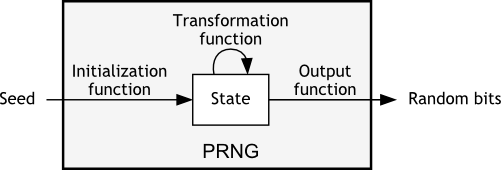
\includegraphics[scale = 0.6]{img/prng_gen.png}
\end{center}

\noindent Thus, the sequence generated by a computer 
algorithm is not truly random, but for a particular length 
of output appears to be random, known as a psuedo random 
sequence.
